%% ------------------------------------------------------------------------- %%
\chapter{Hash Tables}
\label{cap:Hash Tables}

%% ------------------------------------------------------------------- %%
%\begin{itemize}
%\item Define hash table and its operations
%\item Open Addressing Strategies (Linear Probing, Quadratic Probing, ...)
%\item Chaining Strategy (Simple Chaining, Move-to-front ...)
%\item Load factor and resizing/rehashing the table
%\end{itemize}
%% ------------------------------------------------------------------- %%


Hash tables or hash maps is one of the most used applications of hash functions. It is actually so used in computer science that is almost impossible to talk about one without mentioning the other. This data structure consists in associating a \textit{key} to a \textit{value} in a table. That is, given a \textit{key}, it can retrieve the correct \textit{value} for it.

It is considered one of the possible (and one of the best) implementations of a dictionary. It usually has to implement the \textbf{INSERT}, \textbf{FIND} and \textbf{REMOVE} opreations, that can be accessed from outside the dictionary. It usually implements a lot of other private methods. 

This data structure is usually considered very useful among software engineers and computer scientists, although it usually has a linear worst case cost for retrieving, inserting and deleting a key-value pair. That is because it has a constant average cost for those operations.

Moreover, when talking about hash tables we have the problem of key collision, that is when two keys maps to the same hash value. As we saw in the previous chapter, this is collisions are more common than not. To solve that problem, we have several techniques that envolves different tradeoffs. Those techniques are usually divided into two main categories, open addressing and separate chaining. Other problem to consider regarding this data structure is when to resize the hash table, to minimize the chance of collision and the use o memory. For this last one we usually consider a load factor, \( \alpha \), that is the ratio of keys with the available slots.

It is also important to notice that hash tables have applications in different areas of computer science also, like compilers, caches and database indexing.


\begin{figure}[h!]
  \centering
  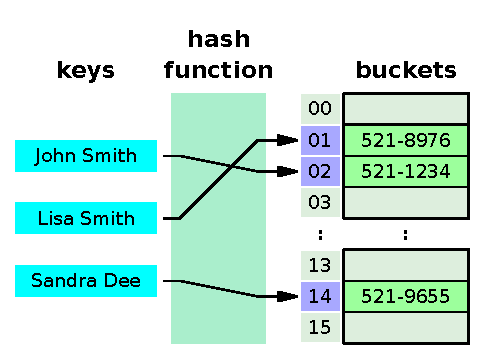
\includegraphics[width=12cm]{figuras/hash-table.pdf}
  \caption{Example of a hash table from string to string, more specifically name to number}
\end{figure}


\section{Open Addressing}

\subsection{Implementing a no collision hash table}

To start I will give an example of a hash table that has a perfect hash function, that has no collisions. For that example we will use open addressing, that basically means that all data will be contained in an array. The operations \textbf{INSERT}, \textbf{FIND} and \textbf{REMOVE} would be very easy to imeplement. For the sake of simplicity, I will assume all the keys are strings. To start lets look at this simple class with dummy methods:

\begin{lstlisting}
class HashTable {
   vector< pair<string, int> > table;
   int m, n;
   
   HashTable() {
      m = 16;
      table.resize(m);
      n = 0;
   }

   unsigned_int hashFunction(string s) {}
   
   void insert(string key, int value) {}

   int find(string key) {}

   void remove(string key) {}

private:
   void resizeIfNecessary() {}
}
\end{lstlisting}

As we can see it is pretty simple. The constructor builds a table of size \( 16 \), and for now we can assume a dinamic resizing every time we have \( 16 \) elements. Later on we will see that this means that we resize every time the load factor, \( \alpha \), is equal to \( 1.00 \). We also can note that at the table part we are storing a pair of key and value, not just value. This is because we may want to retrieve all pairs of the table (like in a regular dictionary). The pairs are usually unordered (If they are not ordered by chance ...), and the iterator has \( O(1) \) step. We will jump the implementation of hashFunction, as already saw plenty of it in the last chapter, so we will go right in for the implementation of \textbf{insert}:

\begin{lstlisting}
void insert(string key, int value) {
  unsigned int idx = hashFunction(key);
  table[idx] = pair<string, int>(key, value);
  n++;
  resizeIfNecessary();
}
\end{lstlisting}

That is pretty simple, that is mostly because we will assume that we will never have a collision, so we just put the key on the position returned by the hash function. The method \textbf{find} is implemented as following:

\begin{lstlisting}
int find(string key) {
  unsigned int idx = hashFunction(key);
  if (table[idx].first == key)
    return table[idx].second;
  return 0;
}
\end{lstlisting}

Also very simple, we always know the value will be in position returned by idx. The \textbf{remove} will be of the same simplicity, as following:

\begin{lstlisting}
void remove(string key) {
  unsigned int idx = hashFunction(key);
  table[idx].first = "";
}
\end{lstlisting}

Here we make the assumption that an empty position has an empty string. We could also carry a boolean (usually called a tombstone) to check if the position is occupied or not. 

\subsection{Formal definition}

\subsection{Linear Probing}

\subsection{Quadratic Probing}

\subsection{When to resize an array}

\subsection{How to delete an entry}

\subsection{Practical advantages of Open Addressing}

\section{Chaining Hashing}

Chaining hashing is the implementation of a hash table using linked lists. On this implementation, each bucket of the table is a pointer to a node of a linked list, that will carry the key value pair in our case. We deal with collisions with this implementation by adding a new node to the end of the list.

This implementation is considered simpler than open addressing, usually because the way of dealing with collisions is clearer. Also it is less system dependant if we consider performance (as we saw ine of the key advantages of open addressing is that it is cache friendly). That is one of the key reasons that C++ uses chaining hashing for its default implementation of unordered\_hash \cite{HashTableProposal}.

Below we can see an implementation of chaining hashing in C++11:

\subsection{Simple Chaining Hashing Algorithm}

\begin{lstlisting}
class Node {
public:
   string key;
   int value;
   Node* nxt;

   Node(string KEY = "", int VALUE = 0, Node* NXT = NULL) {
      key = KEY;
      value = VALUE;
      nxt = NXT;
   }

   ~Node();
};

class ChainingHashTable {
public:
   vector<Node*> table;
   int m, n;
   
   ChainingHashTable() {
      m = 16;
      table.resize(m);
      n = 0;
   }

   unsigned int hashFunction(string s) {...}
   
   void insert(string key, int value) {
      unsigned int idx = hashFunction(key);
      if (table[idx] == NULL) {
         table[idx] = new Node(key, value);
      } else {
         Node* cur = table[idx];
         while (cur->nxt != NULL)
            cur = cur->nxt;
         cur->nxt = new Node(key, value);
      }
      
      n++;
      resizeIfNecessary();
   }
   
   int find(string key) {
      unsigned int idx = hashFunction(key);
      Node* cur = table[idx];

      while (cur->key != key)
         cur = cur->nxt;
      
      if (cur->key == key)
         return cur->value;
      return 0;
   }
   
   void remove(string key) {
      unsigned int idx = hashFunction(key);
      // Empty bucket
      if (table[idx] == NULL)
         return;

      // Remove head of bucket
      if (table[idx]->key == key) {
         Node* rem = table[idx];
         table[idx] = table[idx]->nxt;
         free(rem);
         return;
      }

      // General case
      Node* cur = table[idx];      
      while (cur->nxt != NULL && cur->nxt->key != key)
         cur = cur->nxt;      
      if (cur->nxt != NULL) {
         Node* rem = cur->nxt;
         cur->nxt = rem->nxt;
         free(rem);
      }
      
   }
   
private:
   void resizeIfNecessary() {...};
};
\end{lstlisting}

The implementation has ommited the implementations of \textbf{hashFunction} because that has already been discussed and \textbf{resizeIfNecessary} because that will be discussed later. The methods \textbf{insert}, \textbf{find} and \textbf{remove}


\subsection{Move to front}

\subsection{When to resize an array}

\subsection{How to delete an entry}

\subsection{Practical advantages of Chaining Hashing}

